\chapter{Background}
\label{ch:background}

% Your literature review goes here. \citet{hughes1989functional} discusses the advantages of functional programming by exploring \emph{e.g.}\ lists, trees, and noughts and crosses in a functional programming language. 


As mentioned in \Cref{ch:introduction} there exists research on topic identification in short texts such as social media posts.
Topic analysis on short posts is harder than on longer texts because of the lack of context \cite{}; Twitter posts are limited to xxx
characters, so users tend to attach images, or reference other tweets (via retweeting) to add context that would not be obvious from
the text alone.

\section{Pythia - \cite{Pythia}}
Pythia is an automated system for short text classification. It makes use of Wikipedia structure and articles to identify
topics of posts.
Essentially, "Wikipedia contains articles organized in various taxonomies, called categories". Pythia then goes on to use
this information as their training data as well as handling sparseness in posts on social media.\\

Pythia also demonstrates a method to overcome the lack of context in short texts. They use a method called "Post Enrichment",
which performs i) Named Entity Recognition then ii) Lemmatization and stop word removal. We then use the named entities to query
wikipedia for similar articles that are then appended to the post.\\

Although this method works well in cases where keywords are used, there are cases where no keywords are used, and more context
is needed. Take for example the following tweet:
\newpage
\begin{figure}[htbp]
    \centering
    
\includegraphics[width=0.6\textwidth]{../images/tweet-example.png}
    \caption{Example tweet}
    \label{fig:tweet-example}
\end{figure}

The text, "This is art", gives us no context; What is this tweet about? the best guess I could give
is about some form of art, so we would search wikipedia for articles about art. But in reality this post is about something else.
Lets add some other form of context; add the post the tweet is replying to: "Step up your nade game with @sangalgg and @mahone\_tv
#BLASTPremier". This gives us a lot more context; take the hashtag "BLASTPremier", if we use this for our query we get more relevant
articles:
\newpage

\begin{figure}[htbp]
    \centering
    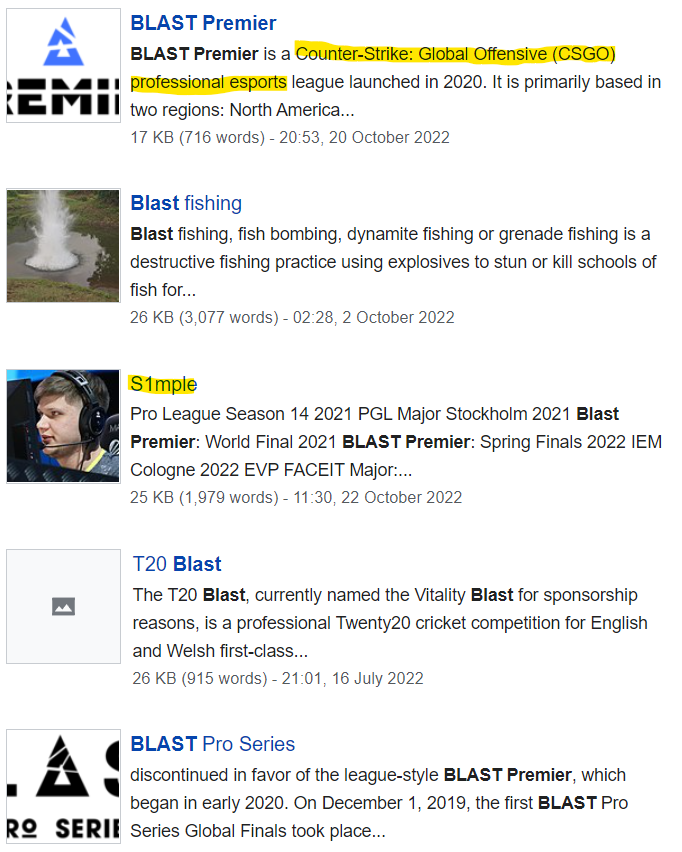
\includegraphics[width=0.6\textwidth]{../images/post-context-example.png}
    \caption{Wikipedia articles related to the hashtag "BLASTPremier"}
    \label{fig:blastpremier}
\end{figure}

We now have a lot of relevant information to append to the post. We could use other information for context as well: Tweet author,
images/media in tweets, retweet information, like information, etc.

\section{Topic tracking of student-generated posts - \cite{TopicTracking}}
This paper proposes a solution for determining valuable information/topics discussed in student forums on online courses.
It uses a model called "Time Information-Emotion Behaviour Model" or otherwise called "TI-EBTM" to detect key topics discussions
, keeping in mind the progress of time throughout the forum.\\
Although this paper specializes in academic online forums, the approaches made could be relevant and useful for this project.

\section{Topic classification of blogs - \cite{husby2012topic}}
This paper uses Distant Supervision - 'an extension of the paradigm used by (\cite{snow}) for exploiting WordNet to extract hypernym (is-a) relations between entitities'
- to get training data via Wikipedia articles. Then trains their own designed model on this data to be able to classify topics via a
multi-class recognition model (69\% accuracy) and via a binary classification model (90\% accuracy).

\section{BERT - \cite{BERT}}
BERT is an acronym for Bidirectional Encoder Represtations from Transformers. It's architecture uses several Transformer encoders
put together.